\documentclass[11pt]{article}
\usepackage[margin=1in]{geometry}
\usepackage{amsmath,amssymb,amsthm,mathtools}
\usepackage{microtype}
\usepackage{tikz}
\usetikzlibrary{arrows.meta}
\usepackage{xcolor}
\definecolor{linkblue}{RGB}{20,55,100}
\usepackage[colorlinks=true,linkcolor=linkblue,citecolor=linkblue,urlcolor=linkblue]{hyperref}
\hypersetup{
  pdftitle={A counterexample to the Monge ansatz for the three-marginal Coulomb cost},
  pdfauthor={OpenAI},
  pdfsubject={Smooth identical marginals with no optimal transport maps for Coulomb and inverse-power Riesz interactions},
  pdfkeywords={multi-marginal optimal transport, Coulomb cost, Riesz cost, Monge ansatz, nonattainment}
}
\usepackage{url}
\newtheorem{theorem}{Theorem}[section]
\newtheorem{lemma}[theorem]{Lemma}
\newtheorem{proposition}[theorem]{Proposition}
\newtheorem{corollary}[theorem]{Corollary}
\theoremstyle{remark}
\newtheorem{remark}[theorem]{Remark}
\newcommand{\R}{\mathbb R}
\newcommand{\Id}{\operatorname{Id}}
\newcommand{\supp}{\operatorname{supp}}
\newcommand{\Leb}{\mathcal L}
\newcommand{\Sym}{\operatorname{Sym}}
\newcommand{\E}{E_*}
\newcommand{\dd}{\,d}
\newcommand{\calH}{\mathcal H}
\newcommand{\calU}{\mathcal U}
\DeclareMathOperator{\diag}{diag}
\setlength{\emergencystretch}{1.5em}
\title{A counterexample to the Monge ansatz\\
for the three-marginal Coulomb cost}
\author{OpenAI}
\date{September 25, 2026}
\begin{document}
\maketitle
\begin{abstract}
We construct a smooth compactly supported probability density on
\(\R^3\), with a smooth compactly supported square root, for which the
three-marginal Coulomb transport minimum is not attained by any pair of
measure-preserving Borel maps. Nevertheless, the Monge and Kantorovich
infima agree: we construct preserving maps whose costs approach the
Kantorovich minimum. For every \(d\ge2\) and \(s>0\), we also construct a
smooth identical marginal with the same nonattainment and equality-of-infima
properties for the inverse-power interaction
\(\sum_{i<j}|x_i-x_j|^{-s}\) on \(\R^d\).
\end{abstract}

\section{The problem and the result}\label{sec:introduction}

For a Borel probability measure \(\mu\) on \(\R^3\), let
\(\Pi(\mu,\mu,\mu)\) denote the probability measures on \((\R^3)^3\)
with all three coordinate marginals equal to \(\mu\). We use the
Coulomb cost
\begin{equation}\label{eq:cost}
 c(x_1,x_2,x_3)=\frac1{|x_1-x_2|}
                 +\frac1{|x_1-x_3|}
                 +\frac1{|x_2-x_3|},
\end{equation}
where \(c=+\infty\) if two coordinates coincide, and write
\[
 \E(\mu)=\inf_{\pi\in\Pi(\mu,\mu,\mu)}\int c\dd\pi.
\]
Here and below \(|\cdot|\) is the Euclidean norm.
A \emph{Monge plan} is a coupling of the form
\((\Id,T_2,T_3)_\#\mu\), where \(T_2,T_3:\R^3\to\R^3\) are
Borel maps and \((T_2)_\#\mu=(T_3)_\#\mu=\mu\).
For a Borel map \(T\), the pushforward is defined by
\(T_\#\mu(A)=\mu(T^{-1}(A))\).
For a map defined on a set of full measure, we use the same notation
for the pushforward of the measure restricted to that set.

The question is whether absolute continuity of \(\mu\), together
with \(\E(\mu)<\infty\), guarantees an optimal Monge plan.
We give a counterexample with additional regularity.

\begin{theorem}\label{thm:main}
There is a nonnegative density \(\rho\) on \(\R^3\) such that
\[
 \int_{\R^3}\rho(x)\dd x=1,\qquad
 \rho\in C_c^\infty(\R^3),\qquad
 \sqrt{\rho}\in C_c^\infty(\R^3),
\]
with the following properties. For \(\mu=\rho\dd x\), the value
\(\E(\mu)\) is finite and is attained by a coupling in
\(\Pi(\mu,\mu,\mu)\), but every pair of Borel maps
\(T_2,T_3:\R^3\to\R^3\) satisfying
\((T_2)_\#\mu=(T_3)_\#\mu=\mu\) obeys
\[
 \int_{\R^3}c\bigl(x,T_2(x),T_3(x)\bigr)\dd\mu(x)>\E(\mu).
\]
The inequality permits the left-hand side to be infinite.
\end{theorem}

The maps in the theorem are arbitrary Borel maps. In particular, the
conclusion concerns existence of any Monge optimizer and includes
maps with no cyclic relation or regularity.
The theorem also excludes optimal symmetrizations of admissible
Monge plans, since permutation averaging preserves their marginals
and Coulomb cost.

\paragraph{History and significance.}
Coulomb multi-marginal transport arises in the strong-interaction
limit of density functional theory. In this setting the description
of optimal configurations by measure-preserving maps is usually
called the Monge or co-motion ansatz. The co-motion formulation was
developed in the strictly correlated electron literature; see Seidl,
Gori-Giorgi and Savin~\cite{SGS2007} and the account by Friesecke,
Gerolin and Gori-Giorgi~\cite{FGG2023}.
The distinction between equality of optimal values and attainment
by maps is essential. Colombo and Di Marino~\cite[author version, Theorem~1.1]{CDM2015} proved
that the Coulomb Kantorovich minimum equals the infimum over
measure-preserving cyclic maps for identical non-atomic marginals.
This provides approximating maps without asserting that a
minimizing map exists. Section~\ref{sec:infima} gives a direct proof of
equality of the two infima for the particular marginal constructed here.

For two particles, Cotar, Friesecke and
Kl{\"u}ppelberg~\cite[arXiv version, Theorem~3.6]{CFK2013}
proved existence and uniqueness of an optimal map for absolutely
continuous marginals in every dimension. For arbitrary particle number
on the line, Colombo, De Pascale and Di Marino~\cite[Theorem~1.1]{CDDM2015}
constructed optimal cyclic maps for identical nonatomic marginals with
finite transport value. Pass~\cite{Pass2013} constructed Coulomb
optimizers that are not induced by maps for radial data; the existence
of such an optimizer does not exclude a different optimizer of Monge
form. Colombo and Stra~\cite{CS2016} gave counterexamples to the
prescribed radial quantile-cyclic constructions. Bindini, De Pascale and
Kausamo~\cite{BDK2022} subsequently constructed smooth densities for
the reduced radial cost of the planar three-particle problem for which
none of the four prescribed maps III, DDI, DID and IDD is optimal.
This radial cost is obtained by minimizing the Coulomb interaction over
angles; it is different from the Coulomb cost on the line.

The general higher-dimensional map-attainment question with at least
three particles is recorded in the 2022 preprint
of~\cite[arXiv version, Theorem~2.4 and the following discussion]{FGG2023}.
The three-particle Coulomb question in \(\R^3\) was still stated as open
in January 2026 by Friesecke~\cite[Section~3.2]{Friesecke2026}.
Theorem~\ref{thm:main} excludes every preserving Borel pair for a smooth
identical marginal. With the particle-density normalization \(n=3\rho\),
one has \(\int n=3\) and \(\sqrt n\in H^1(\R^3)\). Thus the example
belongs to the physical density class \(D_3\)
of~\cite[arXiv version, Eq.~(12)]{FGG2023}. This is a density-regularity
statement; no external potential or ground-state realization is asserted.

Our construction adapts the shared-component splitting mechanism
of Gerolin, Kausamo and Rajala~\cite{GKR2019} for the repulsive
harmonic cost \(-\sum_{i<j}|x_i-x_j|^2\).
For the Coulomb interaction, the additional task is to build two
families of triples with a common supporting potential. We obtain
these families and their supporting inequalities by local calculus.

\paragraph{Idea of the proof.}
The construction has two parts: a geometric condition that forces every
optimal plan onto two prescribed families of triples, and a mass imbalance that
prevents a preserving map from choosing between them.
Let \(B\) be a small ball about zero, and let \(e_1,e_2\) be the first
two coordinate unit vectors. We construct smooth diffeomorphisms \(Y_k,W_k\), for \(k=1,2\), from \(B\) onto small
components near \(e_k,-e_k\), respectively. The two families are
\[
 (x,Y_k(x),W_k(x)),\qquad x\in B,\quad k\in\{1,2\},
\]
together with their coordinate permutations; see
Figure~\ref{fig:components}.

The triples \((0,e_k,-e_k)\) have the same Coulomb cost and the same
central gradient. This allows the two local families to share a
supporting potential on \(B\). Completing this potential on the four
outer components gives an inequality
\(c(x_1,x_2,x_3)\ge u(x_1)+u(x_2)+u(x_3)\), with equality precisely
on the two families. Strict cost gaps exclude the other triples of distinct centers;
the Coulomb singularity excludes repeated components after the
neighborhoods have been made small enough.

For a smooth probability measure \(\nu\) on \(B\), we form the
marginal \(\mu\) by giving the central component measure \(\nu/3\)
and each outer component measure \((Y_k)_\#\nu/6\) or
\((W_k)_\#\nu/6\). Randomly choosing a branch
and permuting its three coordinates then gives an optimal coupling
with this common marginal. Every optimizer must saturate the supporting
inequality. In particular, on the central component, a deterministic
map must choose one of the four branch images. If it chooses a branch
\(H\) on a Borel set \(S\subset B\), it sends mass \(\nu(S)/3\)
into \(H(S)\), which has marginal mass only \(\nu(S)/6\).
This contradicts preservation on every selection set of positive mass.
The exact image-measure relation, rather than the component totals
alone, excludes arbitrarily irregular choices of branch.

\begin{figure}[!b]
\centering
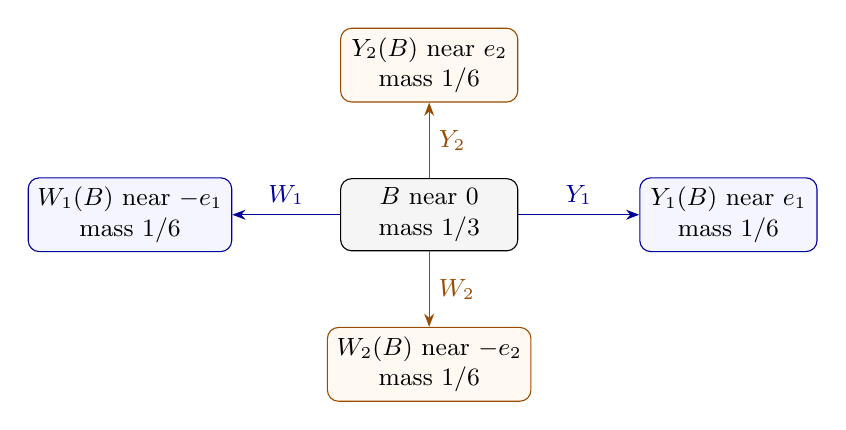
\begin{tikzpicture}[>=Stealth, every node/.style={font=\small},
 component/.style={draw,rounded corners,minimum width=2.25cm,minimum height=.85cm,align=center}]
\node[component,fill=black!4] (B) at (0,0) {$B$ near $0$\\mass $1/3$};
\node[component,draw=blue!60!black,fill=blue!4] (Y1) at (3.8,0)
 {$Y_1(B)$ near $e_1$\\mass $1/6$};
\node[component,draw=blue!60!black,fill=blue!4] (W1) at (-3.8,0)
 {$W_1(B)$ near $-e_1$\\mass $1/6$};
\node[component,draw=orange!60!black,fill=orange!5] (Y2) at (0,1.9)
 {$Y_2(B)$ near $e_2$\\mass $1/6$};
\node[component,draw=orange!60!black,fill=orange!5] (W2) at (0,-1.9)
 {$W_2(B)$ near $-e_2$\\mass $1/6$};
\draw[->,blue!60!black] (B) -- node[above] {$Y_1$} (Y1);
\draw[->,blue!60!black] (B) -- node[above] {$W_1$} (W1);
\draw[->,orange!60!black] (B) -- node[right] {$Y_2$} (Y2);
\draw[->,orange!60!black] (B) -- node[right] {$W_2$} (W2);
\end{tikzpicture}
\caption{Schematic positions of the five disjoint components, with their
marginal masses. Every optimal plan is concentrated on triples joining
a central point to its two images with the same subscript. The arrows
denote local diffeomorphisms, not straight transport trajectories.
For each indicated map \(H\) and Borel set \(S\subset B\),
\(\mu(H(S))=\mu(S)/2\).}
\label{fig:components}
\end{figure}


Sections~\ref{sec:splitting}--\ref{sec:proof} establish the mass obstruction,
construct and certify the two local families, and form the smooth marginal
and an explicit optimizer. Section~\ref{sec:infima} constructs preserving
maps whose costs approach that optimum.
Section~\ref{sec:riesz} extends the construction to every inverse-power
Riesz cost in every Euclidean dimension at least two.

\section{An obstruction to deterministic selection}\label{sec:splitting}

We isolate the measure-theoretic step. A homeomorphism onto an open
image sends Borel sets to Borel sets, since its inverse is
continuous.

\begin{lemma}\label{lem:splitting}
Let \(d\ge2\) be an integer, let \(B\subset\R^d\) be open, let
\(\nu\) be a Borel probability measure with \(\nu(B)=1\), and let
\(H_1,\ldots,H_4:B\to\R^d\) be homeomorphisms onto open images.
Suppose that \(B,H_1(B),\ldots,H_4(B)\) are pairwise disjoint.
Define
\begin{equation}\label{eq:split-measure}
 \mu=\frac13\nu+\frac16\sum_{j=1}^4(H_j)_\#\nu.
\end{equation}
There is no Borel map \(T:\R^d\to\R^d\) such that
\(T_\#\mu=\mu\) and
\begin{equation}\label{eq:selection}
 T(x)\in\{H_1(x),\ldots,H_4(x)\}
 \quad\text{for \(\nu\)-almost every }x\in B.
\end{equation}
\end{lemma}

\begin{proof}
For each \(j\), define the Borel set
\[
 S_j=\{x\in B:T(x)=H_j(x)\}.
\]
Its image \(H_j(S_j)\) is Borel. Pairwise disjointness of the
component images and injectivity of \(H_j\) give
\[
 \mu(S_j)=\frac13\nu(S_j),\qquad
 \mu(H_j(S_j))=\frac16\nu(S_j).
\]
Since \(S_j\subset T^{-1}(H_j(S_j))\), preservation of \(\mu\)
would imply
\[
 \frac13\nu(S_j)
 \le \mu(T^{-1}(H_j(S_j)))
 =\mu(H_j(S_j))
 =\frac16\nu(S_j).
\]
Thus \(\nu(S_j)=0\) for all four indices, contradicting
\eqref{eq:selection}.
\end{proof}

The argument does not require \(\nu\) to be uniform or even
absolutely continuous. Additional points mapped into \(H_j(S_j)\)
can only increase its preimage mass. Matching the total mass of
each component by a partition therefore cannot remove the
obstruction.


\section{Two local Coulomb branches}\label{sec:local}

Put \(a_1=e_1=(1,0,0)\) and \(a_2=e_2=(0,1,0)\).
At each of the two triples \((0,a_k,-a_k)\),
\begin{equation}\label{eq:center-jets}
 c(0,a_k,-a_k)=\frac52,\qquad
 \nabla_xc(0,a_k,-a_k)=0,\qquad
 \nabla_zc(0,a_k,-a_k)=\frac54a_k.
\end{equation}
The equal cost values and vanishing central gradients allow the two
families to share one central potential.

Near each center triple, we use the positive outer point \(y\) as the parameter and find
the central and negative outer points by minimization. Subtracting
suitable concave quadratic potentials in those two coordinates makes
the minimum unique; its value defines the potential at \(y\).
We also require both minimizing coordinates to depend diffeomorphically
on \(y\). We can then invert the central coordinate and obtain both
outer components as diffeomorphic images of a common central set.

\begin{lemma}\label{lem:local}
There are a number \(K>0\), open neighborhoods \(P_0^k,P_k^+,P_k^-\)
of \(0,a_k,-a_k\), respectively, and smooth maps
\(X_k,Z_k:P_k^+\to\R^3\), for \(k=1,2\), with the following
properties:
\begin{enumerate}
 \item Each of \(X_k\) and \(Z_k\) is a diffeomorphism onto its
 open image, and
 \[
  X_k(a_k)=0,\qquad Z_k(a_k)=-a_k.
 \]
 \item Define
 \[
 u_0(x)=\frac52-\frac K2|x|^2,\qquad
 v_k(z)=\frac54a_k\cdot(z+a_k)-\frac K2|z+a_k|^2.
 \]
 There is a smooth function \(w_k:P_k^+\to\R\), with
 \(w_k(a_k)=0\), such that on
 \(P_0^k\times P_k^+\times P_k^-\),
 \begin{equation}\label{eq:local-certificate}
 c(x,y,z)\ge u_0(x)+w_k(y)+v_k(z).
 \end{equation}
 Equality holds if and only if
 \((x,z)=(X_k(y),Z_k(y))\).
\end{enumerate}
\end{lemma}

\begin{proof}
For a parameter \(K>0\), use the potentials in the statement and set
\[
 F_k(x,y,z)=c(x,y,z)-u_0(x)-v_k(z).
\]
By \eqref{eq:center-jets}, its \((x,z)\)-gradient vanishes at the
\(k\)-th center triple. We choose \(K\) to obtain a unique minimizing
pair on a small product neighborhood for each fixed \(y\), and to make each coordinate of the
resulting minimizing pair an invertible function of \(y\).

The Coulomb cost is smooth near both center triples. At the
\(k\)-th center, write
\[
 M_k=D^2_{(x,z)(x,z)}c,\qquad
 N_k=D_y\nabla_{(x,z)}c.
\]
The \((x,z)\)-Hessian of \(F_k\) there is \(M_k+KI_6\), while its
mixed derivative in \(y\) is \(N_k\). For \(h(b)=|b|^{-1}\), \(b\ne0\),
differentiation gives
\begin{equation}\label{eq:pair-hessian}
 D^2h(b)=|b|^{-3}
 \left(3\frac{bb^{\mathsf T}}{|b|^2}-I_3\right).
\end{equation}
This matrix has eigenvalues \(2|b|^{-3},-|b|^{-3},-|b|^{-3}\)
and is therefore invertible. The two \(3\times3\) blocks of \(N_k\) are
\[
 -D^2h(-a_k),\qquad -D^2h(-2a_k),
\]
and hence are both invertible. The matrices \(M_k\) are fixed
symmetric \(6\times6\) matrices. For all sufficiently large \(K\),
both \(M_k+KI_6\) are positive definite. Moreover,
\[
 K(M_k+KI_6)^{-1}N_k
   =(I_6+K^{-1}M_k)^{-1}N_k\longrightarrow N_k.
\]
Invertibility is an open condition on \(3\times3\) matrices, so
we may choose a single \(K\) for which both blocks of
\((M_k+KI_6)^{-1}N_k\) are invertible for each \(k\).

Fix such a \(K\). The implicit function theorem applied to
\(\nabla_{(x,z)}F_k=0\) gives a smooth stationary branch
\[
 \nabla_{(x,z)}F_k(X_k(y),y,Z_k(y))=0,
\]
with the prescribed center values. Differentiating this equation
at \(y=a_k\) gives
\[
 D(X_k,Z_k)(a_k)=-(M_k+KI_6)^{-1}N_k.
\]
The two block invertibilities allow the inverse function theorem
to be applied separately to \(X_k\) and \(Z_k\).
After restricting to one sufficiently small neighborhood of \(a_k\),
both maps are diffeomorphisms onto their open images.

By continuity, the \((x,z)\)-Hessian of \(F_k\) remains positive
definite on a product of sufficiently small open balls around the
three centers. Shrink the \(y\)-ball so that the stationary pair
\((X_k(y),Z_k(y))\) belongs to the product of the other two balls.
For fixed \(y\), this latter product is convex. The positive
definite Hessian makes \(F_k(\cdot,y,\cdot)\) strictly convex on it,
so its stationary pair is its unique minimum there.

Define its minimum value by
\[
 w_k(y)=F_k(X_k(y),y,Z_k(y)).
\]
The preceding minimum property gives
\eqref{eq:local-certificate} with exactly the stated equality set.
The center values in \eqref{eq:center-jets} give \(w_k(a_k)=0\).
All neighborhoods can be restricted further as needed to retain
the separate diffeomorphism properties.
\end{proof}

\section{A supporting inequality on five components}\label{sec:certificate}

The two local inequalities use the same central potential. We can
therefore combine their functions into one potential on five disjoint
components. To identify its entire equality set, we must also show
strict inequality for every component pattern other than permutations
of the two opposite-pair triples \((0,a_k,-a_k)\).

\begin{proposition}\label{prop:certificate}
There are pairwise disjoint open balls \(U_0,U_k^+,U_k^-\) centered
at \(0,a_k,-a_k\), respectively, and a bounded continuous function
\(u:U\to\R\), where
\[
 U=U_0\cup U_1^+\cup U_1^-\cup U_2^+\cup U_2^-,
\]
such that
\begin{equation}\label{eq:certificate}
 c(x_1,x_2,x_3)\ge\sum_{i=1}^3u(x_i)
 \quad\text{on }U^3.
\end{equation}
Equality holds precisely at the triples in \(U^3\) which, after a
permutation, have the form
\begin{equation}\label{eq:contact}
 (X_k(y),y,Z_k(y))\in U_0\times U_k^+\times U_k^-,
 \qquad y\in U_k^+,\quad k\in\{1,2\}.
\end{equation}
The maps \(X_k,Z_k\) are diffeomorphisms on \(U_k^+\), with
\[
 X_k(U_k^+)\subset U_0,\qquad Z_k(U_k^+)\subset U_k^-.
\]
\end{proposition}

\begin{proof}
Use the functions and neighborhoods of Lemma~\ref{lem:local}.
Choose small balls contained in these neighborhoods, taking
\(U_0\) inside both central neighborhoods. On the respective
components define
\[
 u=u_0\ \text{on }U_0,\qquad
 u=w_k\ \text{on }U_k^+,\qquad
 u=v_k\ \text{on }U_k^-.
\]
The balls will be shrunk below. Since the functions are smooth near
their centers, we can first restrict to fixed preliminary balls on
which their absolute values are bounded by one constant \(M>0\).
Take the final balls sufficiently small that their closures are
pairwise disjoint.

At the five centers the values of \(u\) are \(5/2,0,0,0,0\).
For a triple of distinct centers other than a permutation of
\((0,a_k,-a_k)\), there are two
possibilities. If zero is absent, its potential sum is zero and
its cost is positive. If zero is present, the other two centers
come from different opposite pairs. Their cost is
\[
 2+\frac1{\sqrt2}>\frac52,
\]
so again there is a strict gap. There are finitely many such
triples, and the cost and local potentials are continuous near
each one. All these strict inequalities therefore persist on
the corresponding products after sufficiently small restrictions.

For a repeated-center type, two coordinates belong to the same
ball. If all radii are at most \(r\), the distance between those
two coordinates is at most \(2r\), and their pair cost is at least
\(1/(2r)\), with the usual interpretation at coincidence.
Taking \(r\) small enough that \(1/(2r)>3M\) makes the cost
strictly larger than the potential sum on every such product.

The inequalities of Lemma~\ref{lem:local} remain valid when their
domains are restricted, with the same equality characterization.
Permuting a triple leaves both \(c\) and the sum of the three
values of \(u\) unchanged. Thus the two prescribed component types and
their permutations satisfy
\eqref{eq:certificate}, with equality exactly as in
\eqref{eq:contact}; every other type has strict inequality.
Finally, keep \(U_0,U_k^-\) fixed and shrink each \(U_k^+\) once
more. Since \(X_k(a_k)=0\) and \(Z_k(a_k)=-a_k\), continuity
ensures
\[
 X_k(U_k^+)\subset U_0,\qquad Z_k(U_k^+)\subset U_k^-.
\]
All inequalities and diffeomorphism properties survive this
restriction. The function \(u\) is bounded and continuous on
the final disjoint union \(U\).
\end{proof}

We now use the central point as parameter for both equality families.
This gives four diffeomorphisms on one common ball, as required by the
selection obstruction and the construction of the smooth marginal.

\begin{lemma}\label{lem:common-ball}
There is an open ball \(B\) of positive radius centered at zero,
contained in \(U_0\), on which the maps
\[
 Y_k=(X_k|_{U_k^+})^{-1}|_B,\qquad W_k=Z_k\circ Y_k
 \quad(k=1,2)
\]
are well defined and are diffeomorphisms onto open images.
They satisfy
\[
 Y_k(B)\subset U_k^+,\qquad W_k(B)\subset U_k^-,
\]
and every triple \((x,Y_k(x),W_k(x))\), \(x\in B\), is an
equality triple in \eqref{eq:certificate}.
In particular, the five sets
\[
 B,\quad Y_1(B),\quad W_1(B),\quad Y_2(B),\quad W_2(B)
\]
are pairwise disjoint.
\end{lemma}

\begin{proof}
Both \(X_k(U_k^+)\) are open neighborhoods of zero. Choose
a positive-radius ball \(B\) about zero inside their intersection
and \(U_0\). The inverse maps then take \(B\) into \(U_k^+\),
and Proposition~\ref{prop:certificate} gives
\(Z_k(Y_k(B))\subset U_k^-\).
The inverse and composition of the relevant diffeomorphisms are
diffeomorphisms onto open images. The identities
\(X_k(Y_k(x))=x\) and \(W_k=Z_k\circ Y_k\) give equality by
Proposition~\ref{prop:certificate}. Disjointness follows from the
five component balls.
\end{proof}

\section{The marginal and exclusion of every Monge optimizer}
\label{sec:proof}

We now prove Theorem~\ref{thm:main}. Let the balls, maps, and
potential be as in Proposition~\ref{prop:certificate} and
Lemma~\ref{lem:common-ball}. Set
\[
 \calH=\{Y_1,W_1,Y_2,W_2\}.
\]

\paragraph{A smooth marginal.}
Choose a nonnegative function \(g\in C_c^\infty(B)\) with
\(\int_Bg^2\dd x=1\), and let
\(\nu=g^2\dd x\), regarded as a probability measure on \(\R^3\).
Define
\begin{equation}\label{eq:mu}
 \mu=\frac13\nu+\frac16\sum_{H\in\calH}H_\#\nu.
\end{equation}
These coefficients sum to one. For \(H\in\calH\), define
\[
 g_H(y)=
 \begin{cases}
  g(H^{-1}(y))\,|\det DH^{-1}(y)|^{1/2},&y\in H(B),\\
  0,&y\notin H(B).
 \end{cases}
\]
The formula is smooth on \(H(B)\). Its support is contained in
the compact set \(H(\supp g)\subset H(B)\), so extension by zero
is smooth on \(\R^3\). Thus \(g_H\in C_c^\infty(\R^3)\), and
change of variables gives \(H_\#\nu=g_H^2\dd y\).

It follows that \(\mu=\rho\dd x\), where
\[
 \rho=\frac13g^2+\frac16\sum_{H\in\calH}g_H^2.
\]
The functions here are nonnegative and have pairwise disjoint
supports, since their supports lie in the five disjoint
components. Consequently
\[
 \sqrt{\rho}=\frac1{\sqrt3}g
                +\frac1{\sqrt6}\sum_{H\in\calH}g_H.
\]
This proves both asserted smoothness properties, compact support,
and normalization. Also \(\mu(U)=1\) and
\(\mu|_B=(1/3)\nu\).

\paragraph{A finite optimal coupling.}
Sample \(x\) with law \(\nu\), choose \(k\) uniformly from
\(\{1,2\}\), independently of \(x\), and apply an independent
uniform permutation to the three entries of
\[
 (x,Y_k(x),W_k(x)).
\]
Let \(\pi_0\) be the resulting law.
In any fixed coordinate the central point has coefficient \(1/3\),
and each specified outer map has coefficient
\((1/2)(1/3)=1/6\). Hence every coordinate marginal is exactly
\(\mu\).

All sampled triples satisfy \eqref{eq:certificate} with equality.
The boundedness of \(u\) therefore gives
\begin{equation}\label{eq:optimal-value}
 \int c\dd\pi_0=3\int_Uu\dd\mu<\infty.
\end{equation}
Conversely, every \(\pi\in\Pi(\mu,\mu,\mu)\) has
\(\pi(U^3)=1\): each of the three events \(x_i\notin U\)
has probability zero. Integrating \eqref{eq:certificate} yields
\[
 \int c\dd\pi\ge 3\int_Uu\dd\mu.
\]
Thus \(\pi_0\) attains \(\E(\mu)\), and the latter is finite.
Only the inequality on \(U^3\) is used.

For any optimal \(\pi\), the nonnegative slack
\(c(x_1,x_2,x_3)-\sum_i u(x_i)\) on \(U^3\) has integral zero.
Indeed the cost is finite and the potential sum is bounded, so
subtraction and integration are legitimate.
It follows that \(\pi\) is concentrated on the equality triples
in \eqref{eq:contact}.

\paragraph{No optimal maps.}
Suppose that Borel maps \(T_2,T_3\), each preserving \(\mu\),
induce an optimal plan. The preceding equality condition holds
at \((x,T_2(x),T_3(x))\) for \(\mu\)-almost every \(x\), hence
for \(\nu\)-almost every \(x\in B\).

The first coordinate \(x\in B\subset U_0\) is the unique central
coordinate of an equality triple. The remaining coordinates lie
one each in \(U_k^+\) and \(U_k^-\) for some \(k\).
If their values in those components are \(y,z\), then
\(x=X_k(y)\) and \(z=Z_k(y)\).
Injectivity of \(X_k\) forces
\[
 y=Y_k(x),\qquad z=W_k(x).
\]
Allowing either order of these coordinates and either value of
\(k\), we obtain
\[
 T_2(x)\in\{Y_1(x),W_1(x),Y_2(x),W_2(x)\}
 \quad\text{for \(\nu\)-almost every }x\in B.
\]
This contradicts Lemma~\ref{lem:splitting} applied to
\eqref{eq:mu}. Thus no Monge plan attains the minimum, completing
the proof of Theorem~\ref{thm:main}.\qed


\section{Equality of the two infima}\label{sec:infima}

The obstruction above concerns attainment, not the value of the Monge
infimum. We prove this directly for the constructed marginal. The
partition and cost-oscillation argument adapts the approximation method
of Colombo and Di Marino~\cite[author version, Lemma~2.3 and proof of
Theorem~2.1]{CDM2015}. Their general theorem treats the Coulomb singularity
and cyclic maps for identical nonatomic marginals. Here the separated
components allow an elementary proof, including the required Borel maps.

\begin{proposition}\label{prop:equal-infima}
For the probability measure \(\mu\) of Theorem~\ref{thm:main},
\[
 \inf_{\substack{T_2,T_3:\R^3\to\R^3\ \mathrm{Borel}\\
                 (T_2)_\#\mu=(T_3)_\#\mu=\mu}}
 \int c(x,T_2(x),T_3(x))\dd\mu(x)=\E(\mu).
\]
Every pair in this infimum has cost strictly greater than the common
infimum, but pairs with finite cost approach it.
\end{proposition}

The approximation keeps the finite component structure of the optimizer
\(\pi_0\). We partition the components into small cells and prescribe the
mass of a graph plan in each product of three cells to equal that of
\(\pi_0\). Within each product the two plans may differ, but the components
remain separated and the cost oscillation tends to zero with the cell
diameter. To realize the prescribed masses, we split each source cell
into pieces and send each piece into two specified target cells, with
the normalized restriction of \(\mu\) as each target law.
The following elementary transport fact supplies those maps; its proof
is given at the end of the section.

\begin{lemma}\label{lem:borel-transport}
Let \(d\ge2\) be an integer. If \(\alpha\) and \(\beta\) are absolutely
continuous Borel probability measures on \(\R^d\), there is a Borel map
\(Q:\R^d\to\R^d\) such that \(Q_\#\alpha=\beta\).
\end{lemma}

\begin{proof}[Proof of Proposition~\ref{prop:equal-infima}]
Write \(K_0=\supp g\), and let \(K_1,\ldots,K_4\) be its images under
the four maps in \(\calH\). These are nonempty compact sets in the five
disjoint components, and \(\mu(K)=1\) for \(K=\bigcup_{a=0}^4K_a\).
In particular,
\[
 \eta=\min_{a\ne b}\operatorname{dist}(K_a,K_b)>0.
\]
The optimal coupling \(\pi_0\) constructed in Section~\ref{sec:proof}
is supported on products of three distinct component sets.

Fix \(\delta>0\). Partition each \(K_a\) into finitely many Borel cells
of diameter at most \(\delta\), for example by a finite grid of half-open
cubes. Discard the cells of zero \(\mu\)-mass and denote the remaining
cells by \(A_1,\ldots,A_N\). They partition a set of full \(\mu\)-measure
and each belongs to a single \(K_a\). Put
\[
 q_{ijk}=\pi_0(A_i\times A_j\times A_k).
\]
The marginal constraints on \(\pi_0\) read
\[
 \sum_{j,k}q_{ijk}=\mu(A_i),\qquad
 \sum_{i,k}q_{ijk}=\mu(A_j),\qquad
 \sum_{i,j}q_{ijk}=\mu(A_k).
\]
For each fixed \(i\), split \(A_i\) into Borel sets \(B_{ijk}\) of masses
\(q_{ijk}\), ignoring zero-mass pieces. Such a split can be made by
successive first-coordinate slabs: the first-coordinate marginal of
\(\mu|_{A_i}\) is absolutely continuous, so its cumulative distribution
is continuous and takes every value between zero and \(\mu(A_i)\).
Endpoints of the slabs have zero mass; any unused null set is included
in a fixed piece.

For each \(q_{ijk}>0\), Lemma~\ref{lem:borel-transport} supplies maps on
\(B_{ijk}\) sending the probability \(q_{ijk}^{-1}\mu|_{B_{ijk}}\),
respectively, to
\[
 \frac{\mu|_{A_j}}{\mu(A_j)}
 \quad\hbox{and}\quad
 \frac{\mu|_{A_k}}{\mu(A_k)}.
\]
Reset any exceptional values outside the indicated target cell to a
fixed point in that cell. These changes are Borel and occur on null
sets. Glue the maps over the finitely many pieces to obtain \(T_2,T_3\),
and give them a fixed value on the remaining Borel null set in \(\R^3\).
Different source pieces may use the same normalized target law. Their
weights \(q_{ijk}\) add to the full mass of the target cell, so no target
partition is needed. Indeed,
for any Borel set \(D\),
\[
 \mu(T_2^{-1}(D))
 =\sum_{i,j,k:q_{ijk}>0}q_{ijk}
       \frac{\mu(D\cap A_j)}{\mu(A_j)}
 =\sum_j\mu(D\cap A_j)=\mu(D),
\]
and the same calculation proves \((T_3)_\#\mu=\mu\).
The graph coupling \(\pi_\delta=(\Id,T_2,T_3)_\#\mu\) gives each product
\(A_i\times A_j\times A_k\) exactly the mass \(q_{ijk}\).

Whenever \(q_{ijk}>0\), the three cells lie in three distinct component
sets. Thus all pairwise distances in their product are at least
\(\eta\), including after the redistribution within the cells. If
\(x\) and \(y\) are two triples in the same such product, then
\(|x_\ell-y_\ell|\le\delta\) for each coordinate. Consequently
\[
 \left|\frac1{|x_\ell-x_r|}-\frac1{|y_\ell-y_r|}\right|
 \le\frac{2\delta}{\eta^2},
 \qquad |c(x)-c(y)|\le\frac{6\delta}{\eta^2}.
\]
Both costs are finite, bounded by \(3/\eta\) on all active products.
Since \(\pi_\delta\) and \(\pi_0\) have identical masses on these
products, summing their oscillation bounds gives
\[
 \left|\int c\dd\pi_\delta-\int c\dd\pi_0\right|
 \le\frac{6\delta}{\eta^2}.
\]
Letting \(\delta\downarrow0\) proves the required upper bound on the
Monge infimum. The reverse bound follows because every admissible graph
plan is a coupling. Strict nonattainment is Theorem~\ref{thm:main}.
\end{proof}

The argument uses a uniform separation estimate on the approximating
plans themselves; it does not pass the singular Coulomb cost through
weak convergence. No classification or uniqueness of optimal couplings
is needed.

\begin{proof}[Proof of Lemma~\ref{lem:borel-transport}]
We construct a Borel map from each such probability to uniform measure
on \((0,1)^d\), and a Borel map in the reverse direction. Let \(f\) be a
nonnegative Borel probability density. The forward map is Rosenblatt's
successive conditional-distribution transform~\cite{Rosenblatt1952}; we
also give the inverse quantile construction and make the Borel choices
explicit in both directions.

\emph{The forward map.}
We successively transform each coordinate by its conditional distribution
function given the preceding coordinates. Write
\(x_{1:j}=(x_1,\ldots,x_j)\), with \(x_{1:0}\) the empty prefix, and set
\[
 f_{1:j}(x_{1:j})=\int_{\R^{d-j}}f(x_{1:j},z)\dd z
 \quad(1\le j<d),\qquad f_{1:d}=f,\qquad f_{1:0}=1.
\]
The prefix densities are Borel, have integral one, and are finite almost
everywhere. Tonelli's theorem gives
\(\int_\R f_{1:j}(a,r)\dd r=f_{1:j-1}(a)\) for every prefix \(a\),
including the empty prefix when \(j=1\). For \(j=1,\ldots,d\), define
\[
 F_j(a,t)=\frac{\int_{-\infty}^t f_{1:j}(a,r)\dd r}
                 {f_{1:j-1}(a)},\qquad a\in\R^{j-1}.
\]
This formula is used where its denominator belongs to \((0,\infty)\);
on the remaining fibers use instead the fixed distribution function
\(t\mapsto(1+e^{-t})^{-1}\). Thus every fiber is a continuous distribution
function with limits zero and one, and all \(F_j\) are jointly Borel.
For \(j\ge2\), the exceptional prefix fibers have zero probability under
\(f_{1:j-1}(a)\dd a\); there are no exceptional fibers when \(j=1\).

For a random variable with a continuous distribution function \(F\),
the variable \(F(X)\) is uniform on \((0,1)\). Indeed, continuity and the
limits of \(F\) allow a cut at each probability level \(u\in(0,1)\);
any interval on which \(F=u\) has probability zero, and hence
\(\mathbb P(F(X)\le u)=u\). At stage \(j\), this identity and Fubini show
that, conditionally on the preceding original prefix, the new transformed
coordinate is uniform.
It is therefore independent of that prefix, and hence of all preceding
transformed coordinates. A finite induction over \(j=1,\ldots,d\) shows that the Borel map
\[
 R_f(x)=\bigl(F_j(x_{1:j-1},x_j)\bigr)_{j=1}^d
\]
sends \(f\dd x\) to product uniform measure on \((0,1)^d\). Its values lie
in \([0,1]^d\), including on exceptional fibers. This argument does not
require a density to be positive everywhere or a distribution function to
be strictly increasing.

\emph{The reverse map.}
Given independent uniform coordinates, we successively recover the
original conditional laws by quantiles. For each \(j\)
and \(0<u<1\), define
\[
 q_j(a,u)=\inf\{r\in\mathbb Q:F_j(a,r)\ge u\}.
\]
This value is finite, and
\[
 \{(a,u):q_j(a,u)<t\}
 =\bigcup_{\substack{r\in\mathbb Q\\r<t}}
      \{(a,u):F_j(a,r)\ge u\}
\]
proves joint Borel measurability on \(0<u<1\). At \(u=0,1\), define
\(q_j(a,u)=0\). For \(0<u<1\), continuity of \(F_j(a,\cdot)\) gives
\[
 q_j(a,u)\le t\quad\Longleftrightarrow\quad u\le F_j(a,t).
\]
Consequently \(q_j(a,U)\) has distribution function \(F_j(a,\cdot)\)
for uniform \(U\).
For \(u\in[0,1]^d\), recursively set
\[
 z_j=q_j(z_{1:j-1},u_j)\quad(j=1,\ldots,d),
 \qquad S_f(u)=(z_1,\ldots,z_d),
\]
starting with the empty prefix. This finite recursion defines a Borel map.
For independent uniform inputs, induction shows that after step \(j\) the
output prefix has density \(f_{1:j}\): the preceding prefix has density
\(f_{1:j-1}\), its exceptional fibers have probability zero, and on every
other fiber the quantile has the conditional distribution just defined.
Thus \(S_f\) has output law \(f\dd x\).
If \(f\) and \(g\) are densities of \(\alpha\) and \(\beta\), respectively,
then \(S_g\circ R_f\) has the required property.
\end{proof}

\section{Inverse-power Riesz interactions}\label{sec:riesz}

The construction is not specific to the Coulomb exponent or to three
spatial dimensions. For an integer \(d\ge2\) and a real number \(s>0\),
define on \((\R^d)^3\)
\begin{equation}\label{eq:riesz-cost}
 c_s(x_1,x_2,x_3)=\sum_{1\le i<j\le3}|x_i-x_j|^{-s},
\end{equation}
with \(c_s=+\infty\) if two coordinates coincide. For a Borel probability
measure \(\mu\) on \(\R^d\), let \(\Pi(\mu,\mu,\mu)\) now denote the
couplings on \((\R^d)^3\), and write
\[
 E_s(\mu)=\inf_{\pi\in\Pi(\mu,\mu,\mu)}\int c_s\dd\pi.
\]

\begin{theorem}\label{thm:riesz}
For every integer \(d\ge2\) and every real \(s>0\), there is a
nonnegative density \(\rho\) on \(\R^d\) such that
\[
 \int_{\R^d}\rho(x)\dd x=1,\qquad
 \rho\in C_c^\infty(\R^d),\qquad
 \sqrt{\rho}\in C_c^\infty(\R^d),
\]
with the following properties. For \(\mu=\rho\dd x\), the value
\(E_s(\mu)\) is finite and attained by a coupling, but every pair of
Borel maps \(T_2,T_3:\R^d\to\R^d\) with
\((T_2)_\#\mu=(T_3)_\#\mu=\mu\) satisfies
\[
 \int_{\R^d}c_s\bigl(x,T_2(x),T_3(x)\bigr)\dd\mu(x)>E_s(\mu).
\]
The left-hand side may be infinite.
Nevertheless,
\[
 \inf_{\substack{T_2,T_3:\R^d\to\R^d\ \mathrm{Borel}\\
                 (T_2)_\#\mu=(T_3)_\#\mu=\mu}}
 \int c_s(x,T_2(x),T_3(x))\dd\mu(x)=E_s(\mu),
\]
and pairs with finite cost approach this infimum.
\end{theorem}

The density and all local construction constants may depend on
\((d,s)\). The physical Coulomb discussion in
Section~\ref{sec:introduction} refers to the specialization
\(d=3,s=1\); the interaction in \eqref{eq:riesz-cost} is the stated
inverse power, not a logarithmic kernel.

\begin{proof}
Fix \(d\ge2\) and \(s>0\), and put \(a_1=e_1\) and \(a_2=e_2\)
in \(\R^d\). The measure argument already applies in this dimension.
We verify the three properties of the cost that it needs: local
equality families given by diffeomorphisms, strict supporting
inequalities on all other component products, and a uniform
cost-oscillation bound on separated products.

\paragraph{Local branches.}
For \(h_s(b)=|b|^{-s}\), \(b\ne0\), the center jets are
\[
 c_s(0,a_k,-a_k)=2+2^{-s},\qquad
 \nabla_xc_s(0,a_k,-a_k)=0,\qquad
 \nabla_zc_s(0,a_k,-a_k)=s(1+2^{-s-1})a_k.
\]
As before, we keep the positive outer point \(y\) free and minimize
in the other two coordinates. The potentials in Lemma~\ref{lem:local}
are replaced by
\[
 u_0(x)=2+2^{-s}-\frac K2|x|^2,\qquad
 v_k(z)=s(1+2^{-s-1})a_k\cdot(z+a_k)-\frac K2|z+a_k|^2.
\]
The central potential is common to the two branches, and
\(F_k=c_s-u_0-v_k\) has vanishing \((x,z)\)-gradient at each center.
Direct differentiation gives
\[
 D^2h_s(b)=s|b|^{-s-2}
 \left((s+2)\frac{bb^{\mathsf T}}{|b|^2}-I_d\right).
\]
Its radial eigenvalue is \(s(s+1)|b|^{-s-2}\), and its tangential
eigenvalues are \(-s|b|^{-s-2}\), so it is invertible.

At the \(k\)-th center, define \(M_k\) and \(N_k\) as in
Section~\ref{sec:local}, with \(c_s\) in place of \(c\).
The two \(d\times d\) blocks of \(N_k\) are
\(-D^2h_s(-a_k)\) and \(-D^2h_s(-2a_k)\), hence are invertible,
while \(M_k\) is a symmetric \(2d\times2d\) matrix. For sufficiently
large \(K\), both \(M_k+KI_{2d}\) are positive definite and both
\(d\times d\) blocks of \((M_k+KI_{2d})^{-1}N_k\) are invertible, because
\[
 K(M_k+KI_{2d})^{-1}N_k
 =(I_{2d}+K^{-1}M_k)^{-1}N_k\longrightarrow N_k.
\]
One \(K\) works for the two branches. The implicit and inverse function
arguments of Lemma~\ref{lem:local} now give separate local
diffeomorphisms \(X_k,Z_k\) on \(d\)-dimensional neighborhoods.
The cost is smooth near the collision-free center triples; after
shrinking the product balls, the \((x,z)\)-Hessian of \(F_k\) remains positive
definite. Strict convexity on the product of the \(x\)- and \(z\)-balls
therefore gives the same local supporting inequality and exact equality
set, with \(w_k(a_k)=0\).

\paragraph{The supporting inequality and the marginal.}
The five center values of the potential are now
\(2+2^{-s},0,0,0,0\). A distinct-center triple containing zero but
not an opposite pair has cost
\[
 2+2^{-s/2}>2+2^{-s}.
\]
A distinct-center triple without zero has positive cost and potential
sum zero. These finitely many strict gaps persist on small products
by continuity. If two points lie in one ball of radius at most \(r\),
their pair cost is at least \((2r)^{-s}\). This exceeds \(3M\) for
sufficiently small \(r\), where \(M\) bounds the absolute values of
the preliminary potentials. Positivity of the other pair terms and
permutation symmetry of \(c_s\) therefore give the full supporting
inequality and exact contact set described in
Proposition~\ref{prop:certificate}, now in \(\R^d\).
The proof of Lemma~\ref{lem:common-ball} then also applies in \(\R^d\).

On that common ball \(B\), choose a nonnegative
\(g\in C_c^\infty(B)\) with \(\int_B g^2\dd x=1\), and form \(\nu\) and
\(\mu\) by \eqref{eq:mu} using the four resulting diffeomorphisms.
The change-of-variables construction in Section~\ref{sec:proof},
now with \(d\)-dimensional Jacobians, gives the same smooth compactly
supported density and square root: each image function is supported
compactly inside its open component, and the five supports are
disjoint. The same random choice of a branch and permutation gives
an optimal coupling \(\pi_0\) with the three marginals equal to
\(\mu\). The bounded supporting potential proves its cost is finite
and forces every optimal coupling onto the contact set. Applying
Lemma~\ref{lem:splitting} to the four branch maps then excludes
every marginal-preserving Borel pair, exactly as in
Section~\ref{sec:proof}.

\paragraph{Approximation by preserving maps.}
The five compact component sets have a positive mutual separation
\(\eta\), and \(\pi_0\) uses only products of three distinct components.
Repeat the cell partition and redistribution from the proof of
Proposition~\ref{prop:equal-infima} in \(\R^d\), using
Lemma~\ref{lem:borel-transport}. The first-coordinate marginals used
to split the cells are absolutely continuous by Fubini in every such
dimension. The redistribution gives a graph coupling
\(\pi_\delta\) of a preserving Borel pair with the same mass as
\(\pi_0\) on each product of cells of diameter at most \(\delta\).
Every active product still has all pair distances at least \(\eta\).
For two triples \(x,y\) in one such product, the scalar mean value
theorem gives
\[
 \left||x_\ell-x_r|^{-s}-|y_\ell-y_r|^{-s}\right|
 \le 2s\delta\,\eta^{-s-1},\qquad
 |c_s(x)-c_s(y)|\le6s\delta\,\eta^{-s-1}.
\]
Both costs are bounded by \(3\eta^{-s}\) on the active products.
Summing their oscillations against the common product masses yields
\[
 \left|\int c_s\dd\pi_\delta-\int c_s\dd\pi_0\right|
 \le6s\delta\,\eta^{-s-1}\longrightarrow0.
\]
The reverse inequality for the infima holds because every graph plan
is a coupling. This proves the final assertion. In particular, no
restriction relating \(s\) to \(d\) is needed: the optimizer and
these approximating plans stay away from all collisions.
\end{proof}


\bibliographystyle{plain}
\bibliography{references}
\end{document}
